%%%%%%%%%%%%%%%%%%%%%%%%%%%%%%%%%%%%%%%%%%%%%%%%%%%%%%%%%%%%%%%%%%%%%%%%%%%

\documentclass{standalone}

\usepackage{amsmath}
\usepackage{mathptmx}
\usepackage{pgfplots}
\usetikzlibrary{external}
\tikzexternalize{ecoli}
\pgfplotsset{compat=1.16}

%% IEEE uses Times Roman font, so we'll default to Times.
%% These three commands make up the entire times.sty package.
\renewcommand{\rmdefault}{ptm}
\renewcommand{\ttdefault}{pcr}
\normalfont\selectfont

\begin{document}

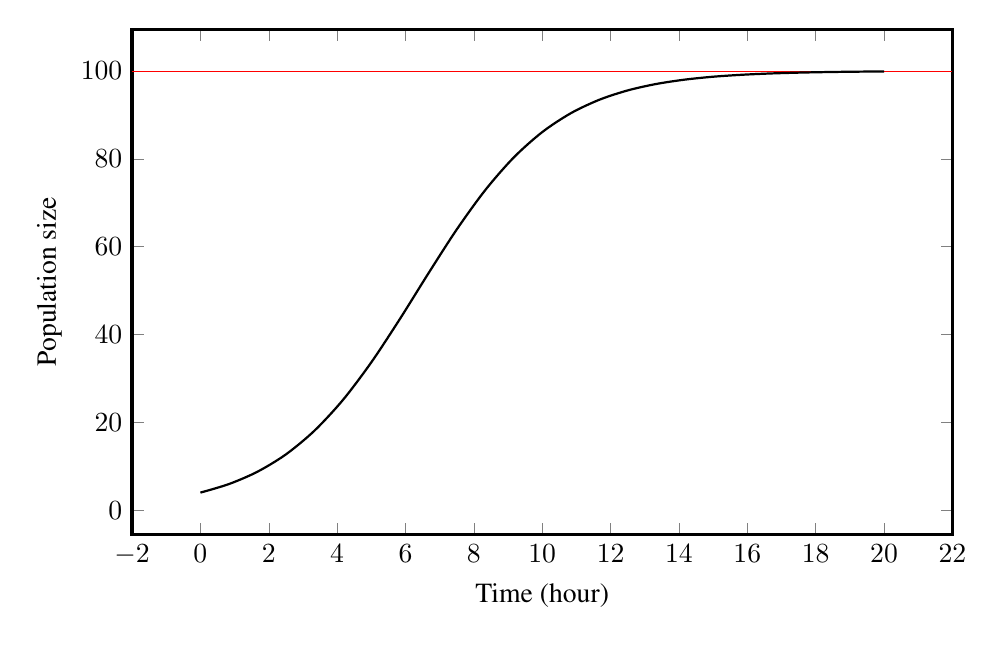
\begin{tikzpicture}
\tikzset{%%
  every mark/.append style={scale=1.0},%%
  scale=1.0%%
}
\pgfplotsset{%%
  every axis/.append style={font=\normalsize}%%
}
%%
\begin{axis}[%%
  axis line style=very thick,%%
  enlargelimits=true,%%
  height=8cm,%%
  legend cell align=left,%%
  legend pos=north west,%%
  plotStyle/.style={%%
    domain=0:20,%%
    mark=none,%%
    smooth,%%
    thick%%
  },%%
  width=12cm,%%
  %% x axis
  xlabel={\normalsize Time~(hour)},%%
  %% y axis
  ylabel={\normalsize Population size}%%
]
%%
%%
%% Horizontal line through y = 100.
\draw[ultra thin,red] (axis cs:\pgfkeysvalueof{/pgfplots/xmin},100) -- (axis cs:\pgfkeysvalueof{/pgfplots/xmax},100);
%%
%%
\addplot+ [plotStyle,black]
{100 / (1 + 24*exp(-x/2))};
\end{axis}
\end{tikzpicture}

\end{document}
